
\documentclass{article}
\usepackage[backend=biber,style=ieee,sorting=none]{biblatex}
\addbibresource{RecommendationBib.bib}
\usepackage{amsmath}
\usepackage{amssymb}
\usepackage{graphicx}
\usepackage{multirow}
\usepackage{booktabs}
\usepackage{subcaption}
\usepackage{caption}
\usepackage{float}
\usepackage{geometry}
\geometry{margin=1in}
\usepackage{algorithm}
\usepackage{algorithmic}
\usepackage{tikz}
\usetikzlibrary{positioning, shapes.geometric, arrows.meta, fit}


\tikzset{
  process/.style={rectangle, draw=blue!60, fill=blue!10, very thick, minimum height=1cm, minimum width=3.5cm, text centered, rounded corners},
  io/.style={rectangle, draw=blue!60, fill=blue!5, very thick, minimum height=1cm, minimum width=4cm, text centered, rounded corners},
  arrow/.style={thick,->,>=Stealth}}

%opening
\title{Bayesian Clustering with User-Side Information for Streaming Recommender Systems: Addressing Data Sparsity and Cold-Start with Provable Convergence}
\author{}

\begin{document}

\maketitle

\begin{abstract}
Collaborative filtering, a popular technique in recommendation systems, faces primary challenges: data sparsity, cold-start limitations, and an inability to adapt to streaming data in real-world environments. Although existing heuristic and distance-based approaches partially address streaming scenarios, they lack theoretical rigor and fail to leverage evolving user-item interactions effectively. This study introduces a novel Bayesian clustering framework that integrates user-side information with probabilistic priors to overcome these challenges. 
The proposed clustering method reduces the impact of rating matrix sparsity by leveraging prior knowledge for streaming data. Furthermore, incorporating user-side information mitigate the effects of the cold-start problem on prediction accuracy.
The convergence of the proposed clustering method is established in this study through the proof that the Hessian matrix of its objective function is positive definite. Empirical validation demonstrates a faster convergence rate of proposed method compared to the Fuzzy C-Means. The experimental results on real-world streaming datasets (MovieLens, yelp) indicate that the proposed method, in addition to overcoming the limitations, achieves higher accuracy in predicting user ratings than other methods. By integrating Bayesian inference with the ability to adapt to streaming data, this study addresses key limitations in current recommender systems research. 

\textbf{Keywords}:Bayesian Clustering, Streaming Data, Collaborative Filtering, Cold-Start Mitigation, Data Sparsity, Convergence Analysis, Side Information, Recommendation Systems.
\end{abstract}

\section{Introduction}
Every piece of knowledge builds upon another, and the understanding of any truth requires awareness of its foundation. 
Recommender systems, much like the evolution of knowledge, build upon prior information to refine and enhance decision-making. These systems aim to maximize user satisfaction by generating a list of the most relevant and personalized items. Given their significance, extensive research has been conducted in this domain, exploring various methodologies to improve recommendation quality. Each approach relies on different sources of information, benefiting from past interactions to predict future preferences. However, much like gaps in historical knowledge challenge understanding, recommender systems also struggle with incomplete data, cold-start issues, and the dynamic nature of evolving user-item interactions.

Recommender systems aim to enhance user satisfaction by generating a list of the most relevant and personalized items. Given their significance, extensive research has been conducted in this domain, exploring various methodologies for improving recommendation quality. Each approach leverages different types of information and comes with its own advantages and limitations.  

\underline {\textbf{challenge 1:}}
Despite substantial advancements, recommender systems still face critical challenges rooted in the nature of user–item interaction data, including the cold-start problem, data sparsity, and imbalance \cite{li2024recent, rama2019deep}. These limitations reduce prediction accuracy, preventing the system from effectively tailoring recommendations to user preferences.

\underline{\textbf{challenge 2:}}
 Many existing models assume a static dataset, whereas in real-world scenarios, data arrives continuously in a streaming manner. The ability to handle such dynamic data influx remains a pressing challenge, as most traditional approaches lack adaptability to evolving user-item interactions.  

To address these limitations, this paper proposes a Bayesian clustering framework for streaming recommendation that addresses sparsity and cold-start by leveraging user-side information. we derive an update rule with provable convergence guarantees, ensuring that the model adapts stably as the data stream evolves. This model enhances both the accuracy and adaptability of recommender systems.

The remainder of this paper is organized as follows. Section 2 reviews the literature on content-based, collaborative methods, with a detailed focus on clustering-based CF and the use of side information. Section 3 details the proposed method, including the clustering techniques employed and their integration into the recommender system. Section 4 presents the evaluation of the system’s performance, offering a comparative analysis with existing methods. Finally, Section 5 concludes the study and suggesting directions for future research.

\section{Related Work}
Methods in recommender systems are included three main categories content-based methods, collaborative Filtering(CF), and Hybrid methods \cite{aljunid2025collaborative}. Content-based methods generate recommendations solely based on a user's past behavior and interests, without considering other users' interactions. While simple to implement, they provide a limited selection of similar items and fail to leverage relationships between users. 

Collaborative filtering focuses on user-item interactions rather than item characteristics, recommending items based on the preferences of similar users. This approach enables more diverse and personalized recommendations by utilizing shared user behaviors and preferences \cite{isinkaye2023matrix}. Collaborative methods have two types of algorithms, memory-based and model-based.

In memory-based methods, which are also called neighborhood-based methods, the relationship between users and items is investigated. User-based \cite{zhao2010user,valcarce2019collaborative} or item-based \cite{sarwar2001item,fu2018attention} similarity is considered to predict the user's rating of items that he has not seen before. The primary limitation of memory-based methods is their reliance on loading the entire rating matrix into memory for each prediction, making them inefficient for large-scale datasets in terms of time and memory usage. 

Model-based methods address this issue by employing a predictive model  based on past user-item interactions. Various machine learning algorithms can be utilized in model-based approaches to enhance recommendation accuracy and efficiency. These mainly includes approaches like Matrix factorization \cite{isinkaye2023matrix,shi2020user,yang2018enhancing, behera2023mixed}, Bayes classifier \cite{valdiviezo2019collaborative}, neural networks \cite{wang2015collaborative,angel2022deep,li2017collaborative}.
This paper focuses on common challenges in recommender systems and clustering algorithms. Clustering techniques are commonly used to mitigate the sparsity problem and improve the scalability of CF methods. By grouping users or items with similar characteristics, clustering-based CF systems enhance recommendation performance while reducing computational complexity. 
\begin{itemize}
\item[a) ] Clustering-based Collaborative Filtering \\
Clustering algorithms such as k-means\cite{dakhel2011new, zahra2015novel, ranjan2018category, kant2017leaderrank} and FCM\cite{birtolo2013advances} are widely utilized in recommender systems. Studies have explored various user clustering approaches, including Bayesian matrix factorization \cite{bobadilla2018recommender}, evolutionary clustering that adapts user states over time \cite{liji2018improved}, and weighted clustering that assigns higher importance to users with more interactions \cite{salah2015dynamic}. In \cite{katarya2018recommender}, a hybrid method used gray wolf optimization for initializing clusters, followed by fuzzy c-means (FCM) for user classification based on rating similarity .
Similarly, for item clustering, in \cite{deng2019novel}, an improved Kullback-Leibler divergence is employed to measure item similarity based on probability distributions. In \cite{kant2017leaderrank}, the k-means algorithm is utilized to cluster items, and an item's score is predicted solely based on the average scores of other items within the same cluster. Several methods have been proposed for clustering both users and items. Other approaches include power fuzzy clustering using an exponential fitness function to refine membership \cite{treerattanapitak2012exponential} and network-based clustering where evolving statuses lead to stable groups \cite{chen2017evolutionary}. Clustering via the QUBIC (A Qualitative Biclustering algorithm) in \cite{singh2018impact}, aim to group similar users and items effectively. \cite{science2018dynamic} constructs a network that integrates user characteristics, item features, and temporal information, subsequently applying a dynamic evolutionary clustering algorithm.

Several advanced clustering-aware approaches such as \cite{rajput2025nsga}, proposes an NSGA-II-optimized deep autoencoder framework improve multi-criteria recommendations by optimizing model parameters through a multi-objective approach, addressing data sparsity and non-linearity. \cite{li2025self} presents a self-supervised graph Transformer (SGTN) that improves user-item representations by encoding ratings and applying contrastive learning. It focuses on capturing social and collaborative relationships through decentralized graphs and edge-aware attention. Although not explicitly designed for clustering, it enhances user embeddings, enabling dynamic and context-sensitive user-item grouping in recommendation systems. In \cite{qian2025ifm} a framework that uses adversarial features from multiple models is proposed to improve transferability and enhance user-item representations. It refines embeddings by reducing noise and improving cluster separability, offering a strategy for robust clustering in dynamic recommendation systems. \cite{he2025fedai} presents FedAI, a federated recommendation system that combines spectral clustering and K-means to group users while ensuring privacy. High-order interactions enhance embeddings, improving clustering in decentralized settings without accessing raw data.


\item[b) ] Clustering based on User-side Information \\ 
While clustering-based methods address scalability and sparsity issues in the score matrix, the high dimensionality of user-item data makes them computationally expensive. To mitigate this, many approaches leverage side information as clustering features, significantly reducing the feature space and improving efficiency. \cite{liji2018improved} employs user attributes such as age, gender, and residence to calculate feature distances for clustering. Similarly, \cite{chen2019n2vscdnnr} forms a bipartite user-item graph and converts each node into a vector before clustering. Additionally, \cite{zhao2017coarse} clusters users based on social network labels and items via a bipartite graph, \cite{sheugh2018novel} creates a two-dimensional similarity graph of users for clustering, and \cite{wasid2018clustering} incorporates social information alongside the score matrix to enhance user clustering. Gong et al. \cite{gong2010collaborative} leveraged both explicit ratings and implicit user behavior to improve similarity measurements. Lu et al. \cite{lu2021novel} addressed the sparsity problem in user-item interactions by grouping items with similar features, thereby aligning recommendations more closely with user interests. Additionally, Wasid et al. \cite{wasid2018improved} refined traditional collaborative filtering through a multi-criteria clustering approach, which integrates various aspects of user preferences to yield more diverse and accurate recommendations. Additionally, Mahalanobis distance is employed to measure the similarity between users' score vectors, taking into account not only the given scores but also their variance and covariance \cite{deng2019neural} used variational autoencoders and side information to mitigate data sparsity and the cold start problem. 

\item[c) ] Recommendation in Streaming Data Environment \\
Furthermore, most of clustering-based methods often do not consider streaming data, making them less effective in dynamic environments. With the increasing need for real-time recommendations, online recommender systems have become essential for handling streaming data. These systems must efficiently update user preferences and item interactions as new information becomes available. Recommender systems in e-commerce and digital service platforms must continuously process new users and items, making real-time data handling essential. However, most existing systems rely on fixed datasets for evaluation, limiting their applicability in dynamic environments. Traditional content-based and memory-based collaborative filtering methods require loading all data into memory, making them unsuitable for streaming data. In contrast, model-based collaborative filtering, particularly matrix decomposition methods like ALS and SGD, allows incremental updates. While these methods address some streaming challenges, they remain computationally expensive and risk losing information during model updates. Clustering-based recommender systems for streaming data mainly rely on heuristics without leveraging prior knowledge, limiting their effectiveness. For instance, distance-based clustering adjusts noisy data positioning \cite{georgieva2008dynamic}, as well as a density-based method updates clusters dynamically using local averages\cite{baruah2012evolving}. In \cite{das2007google} an online model proposed for Google News, continuously updates recommendations based on user interactions, ensuring that personalized news suggestions remain relevant. A streaming matrix‐factorization framework proposed in \cite{jakomin2020simultaneous} that incrementally fuses multiple heterogeneous data streams to continuously adapt latent user‐item representations and mitigate both data sparsity and cold‐start issues. While online recommender systems rely on user feedback, new users, and new items for updates, many clustering-based methods struggle with streaming data. Integrating online learning into clustering-based collaborative filtering can improve adaptability in dynamic environments.
\end{itemize}

One of the primary strategies for mitigating data sparsity is cluster-based collaborative filtering. Clustering-based recommender systems can enhance recommendation reliability while maintaining lower computational complexity. Despite the benefits of clustering-based CF methods, challenges remain. Feature selection for clustering is a critical issue, as high-dimensional user-item matrices can lead to the curse of dimensionality. Conversely, clustering based on side features alone may not accurately capture user interests, reducing prediction accuracy. In addition, deal with streaming data, making them effective in dynamic environments is rally important.

To address these limitations, a Bayesian clustering model is introduced, incorporating prior knowledge for streaming data clustering. Unlike traditional clustering approaches, this method dynamically updates user and item clusters as new interactions occur. By combining user ratings with side features, the model improves personalization, incorporates real-time updates to handle user feedback, new users, and alleviates the cold start problem by leveraging additional user information beyond the rating matrix. Experimental results demonstrate that this approach outperforms existing clustering-based CF models in terms of accuracy and efficiency, making it well-suited for real-time recommendation systems. 









\section{Proposed Method}
\label{sec:proposed_method}




\subsection{Problem Formulation through Bayesian Latent Filtering}
\label{subsec:bayesian_latent_filtering}

Let \(x\in\mathcal{X}\) denote an incoming item. The goal is to infer which candidate item-set
\[
\mathcal{S}_j\subseteq\mathcal{X},\qquad j=1,\ldots,K,
\]
is most relevant to \(x\). Each set \(\mathcal{S}_j\) is represented by a latent descriptor
\[
\theta_j=(\mu_j,\Sigma_j),
\]
where \(\mu_j\) and \(\Sigma_j\) describe the center and dispersion of the latent representation of the items belonging to \(\mathcal{S}_j\).

Instead of directly mapping \(x\) to \(\mathcal{S}_j\), we introduce an intermediate latent filtering layer. First, the incoming item is encoded into a latent vector
\[
\mathbf{z}(x)=\phi(x)\in\mathbb{R}^{d}.
\]
Then, the model estimates the posterior involvement of \(x\) in each hidden component \(c_i\), \(i=1,\ldots,C\):
\[
q_i(x)
\triangleq
P(c_i\mid x)
=
P(c_i\mid \mathbf{z}(x)).
\]
This posterior plays the role of a Bayesian filter over the latent space.

To compute \(q_i(x)\), each hidden component \(c_i\) is represented by a latent prototype and covariance
\[
\psi_i=(\mathbf{m}_i,\Lambda_i),
\]
and the likelihood of the encoded item under component \(c_i\) is modeled as
\[
p(\mathbf{z}(x)\mid c_i)
=
\mathcal{N}\!\left(\mathbf{z}(x);\mathbf{m}_i,\Lambda_i\right).
\]
Hence, by Bayes' rule,
\[
q_i(x)
=
P(c_i\mid x)
=
\frac{
	\rho_i\,\mathcal{N}\!\left(\mathbf{z}(x);\mathbf{m}_i,\Lambda_i\right)
}{
	\sum_{\ell=1}^{C}
	\rho_\ell\,\mathcal{N}\!\left(\mathbf{z}(x);\mathbf{m}_\ell,\Lambda_\ell\right)
},
\]
where \(\rho_i=P(c_i)\) is the prior probability of the \(i\)-th hidden component.

After this filtering step, the relevance of the hidden component \(c_i\) to the candidate set \(\mathcal{S}_j\) is evaluated through the latent descriptor \(\theta_j\). In particular, the prototype \(\mathbf{m}_i\) is assessed under the distribution associated with \(\mathcal{S}_j\):
\[
f(\mathbf{m}_i\mid \theta_j)
=
\mathcal{N}(\mathbf{m}_i;\mu_j,\Sigma_j).
\]
The correct Gaussian form is
\[
f(\mathbf{m}_i\mid \theta_j)
=
\frac{1}{(2\pi)^{d/2}|\Sigma_j|^{1/2}}
\exp\left(
-\frac{1}{2}
(\mathbf{m}_i-\mu_j)^T
\Sigma_j^{-1}
(\mathbf{m}_i-\mu_j)
\right).
\]
Therefore, using Bayes' rule, the posterior association between the set descriptor \(\theta_j\) and the hidden component \(c_i\) is
\[
f(\theta_j\mid \mathbf{m}_i)
=
\frac{
	f(\mathbf{m}_i\mid \theta_j)\,P(\theta_j)
}{
	\sum_{r=1}^{K}
	f(\mathbf{m}_i\mid \theta_r)\,P(\theta_r)
}.
\]

The complete inference chain is therefore
\[
x
\longrightarrow
\mathbf{z}(x)=\phi(x)
\longrightarrow
P(c_i\mid x)
\longrightarrow
f(\theta_j\mid \mathbf{m}_i)
\longrightarrow
\mathcal{S}_j .
\]
Accordingly, the relevance score of the incoming item \(x\) to the candidate set \(\mathcal{S}_j\) is obtained by marginalizing over all hidden components:
\[
R_j(x)
=
\sum_{i=1}^{C}
P(c_i\mid x)\,
f(\theta_j\mid \mathbf{m}_i).
\]
Finally, the most relevant set is estimated as
\[
\widehat{j}
=
\arg\max_{j}
R_j(x)
=
\arg\max_{j}
\sum_{i=1}^{C}
P(c_i\mid x)\,
f(\theta_j\mid \mathbf{m}_i),
\]
and the recommended set is
\[
\widehat{\mathcal{S}}(x)=\mathcal{S}_{\widehat{j}}.
\]

This formulation separates the two probabilistic roles of the latent space. The term \(P(c_i\mid x)\) measures how the incoming item activates hidden components, while \(f(\theta_j\mid \mathbf{m}_i)\) measures how each hidden component supports a candidate recommendation set.







% Required TikZ libraries:
% \usetikzlibrary{positioning,arrows.meta,calc,fit}

\subsection{Bayesian Latent Filtering View}
\label{subsec:bayesian_latent_filtering_view}

Let \(x\in\mathcal{X}\) denote an incoming item. The purpose of the recommender is to estimate the most relevant candidate set
\[
\mathcal{S}_j\subseteq\mathcal{X},
\qquad j=1,\ldots,K,
\]
for the input item \(x\). Each set \(\mathcal{S}_j\) is represented by a latent descriptor
\[
\theta_j=(\mu_j,\Sigma_j).
\]

We introduce a hidden component variable
\[
c_i,\qquad i=1,\ldots,C,
\]
where \(c_i\) denotes the \(i\)-th internal latent cluster or hidden component. Each hidden component is represented by a prototype
\[
\mathbf{m}_i\in\mathbb{R}^{d}.
\]
Thus, \(c_i\) is the latent event, while \(\mathbf{m}_i\) is its continuous representative in the latent space.

The input item is first mapped into a latent representation
\[
\mathbf{z}(x)=\phi(x).
\]
The Bayesian filtering stage estimates the posterior activation of each hidden component:
\[
q_i(x)
=
P(c_i\mid x)
=
\frac{
	\rho_i\,p(\mathbf{z}(x)\mid c_i)
}{
	\sum_{\ell=1}^{C}
	\rho_\ell\,p(\mathbf{z}(x)\mid c_\ell)
},
\]
where \(\rho_i=P(c_i)\) is the prior probability of the \(i\)-th hidden component.

If the latent representation of component \(c_i\) is modeled by a Gaussian distribution centered at \(\mathbf{m}_i\), then
\[
p(\mathbf{z}(x)\mid c_i)
=
\mathcal{N}\big(\mathbf{z}(x);\mathbf{m}_i,\Lambda_i\big).
\]

After the hidden component is inferred, the model evaluates how strongly this internal component supports each candidate set \(\mathcal{S}_j\). This is expressed as
\[
f(\theta_j\mid c_i).
\]
Since \(c_i\) is represented by its prototype \(\mathbf{m}_i\), this posterior can be computed through
\[
f(\theta_j\mid c_i)
\equiv
f(\theta_j\mid \mathbf{m}_i).
\]
Using Bayes' rule, we obtain
\[
f(\theta_j\mid \mathbf{m}_i)
=
\frac{
	f(\mathbf{m}_i\mid \theta_j)P(\theta_j)
}{
	\sum_{r=1}^{K}
	f(\mathbf{m}_i\mid \theta_r)P(\theta_r)
}.
\]
Here,
\[
f(\mathbf{m}_i\mid \theta_j)
=
\mathcal{N}(\mathbf{m}_i;\mu_j,\Sigma_j),
\]
that is,
\[
f(\mathbf{m}_i\mid \theta_j)
=
\frac{1}{(2\pi)^{d/2}|\Sigma_j|^{1/2}}
\exp\left(
-\frac{1}{2}
(\mathbf{m}_i-\mu_j)^T
\Sigma_j^{-1}
(\mathbf{m}_i-\mu_j)
\right).
\]

Therefore, the relevance score of the incoming item \(x\) to the candidate set \(\mathcal{S}_j\) is
\[
R_j(x)
=
\sum_{i=1}^{C}
P(c_i\mid x)\,
f(\theta_j\mid c_i).
\]
Finally, the estimated recommendation set is
\[
\widehat{\mathcal{S}}(x)
=
\mathcal{S}_{\widehat{j}},
\qquad
\widehat{j}
=
\arg\max_{j}
\sum_{i=1}^{C}
P(c_i\mid x)\,
f(\theta_j\mid c_i).
\]

\begin{figure}[t]
	\centering
	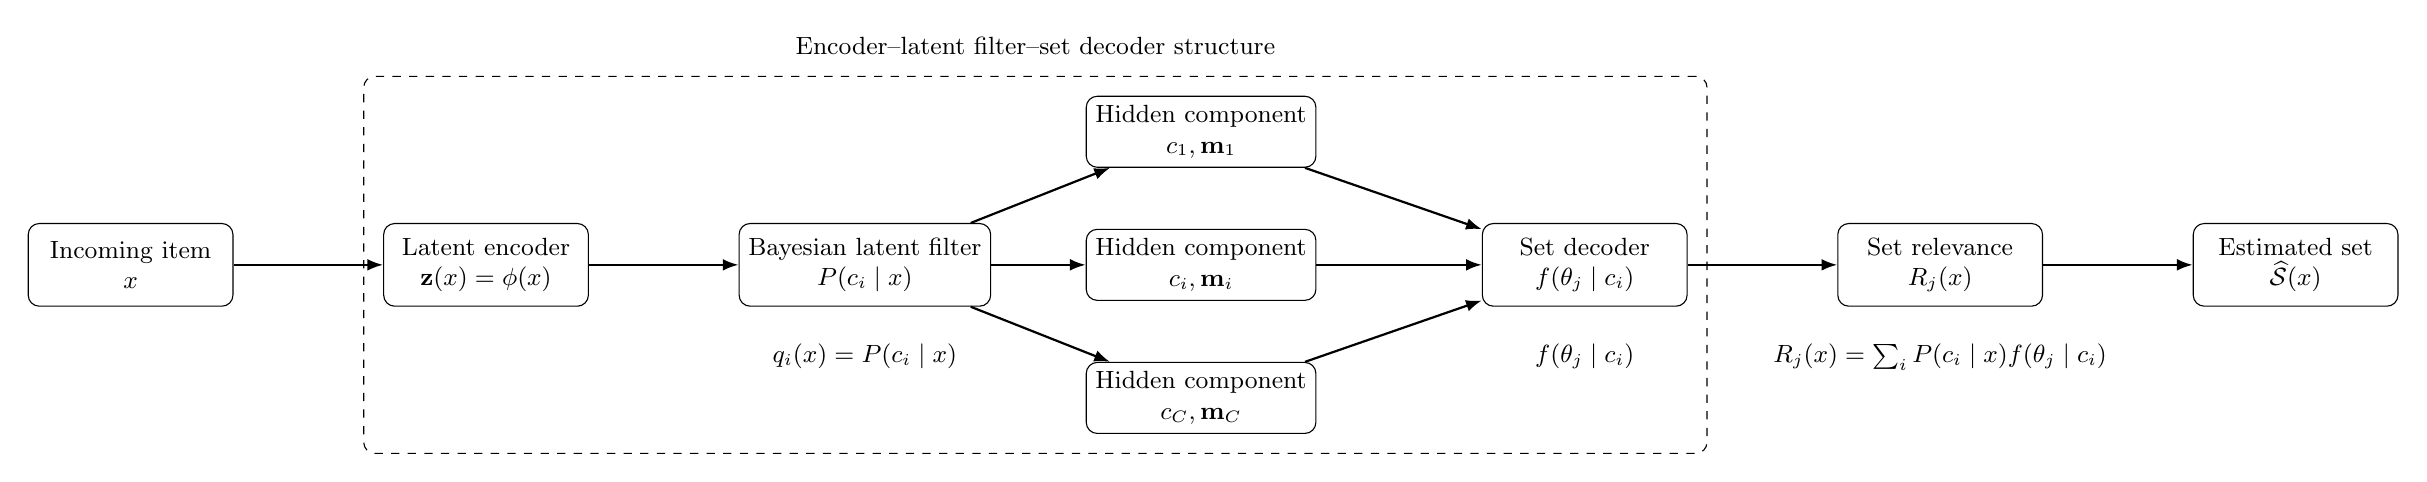
\begin{tikzpicture}[
		node distance=1.55cm and 1.9cm,
		box/.style={
			draw,
			rounded corners,
			align=center,
			minimum width=2.6cm,
			minimum height=1.05cm,
			font=\small
		},
		smallbox/.style={
			draw,
			rounded corners,
			align=center,
			minimum width=2.25cm,
			minimum height=0.9cm,
			font=\small
		},
		arrow/.style={-{Latex[length=2mm]}, thick},
		dashedbox/.style={
			draw,
			dashed,
			rounded corners,
			inner sep=7pt
		}
		]
		
		\node[box] (x) {Incoming item\\ \(x\)};
		\node[box, right=of x] (enc) {Latent encoder\\ \(\mathbf{z}(x)=\phi(x)\)};
		\node[box, right=of enc] (filter) {Bayesian latent filter\\ \(P(c_i\mid x)\)};
		
		\node[smallbox, above right=0.7cm and 1.2cm of filter] (c1) {Hidden component\\ \(c_1,\mathbf{m}_1\)};
		\node[smallbox, right=1.2cm of filter] (ci) {Hidden component\\ \(c_i,\mathbf{m}_i\)};
		\node[smallbox, below right=0.7cm and 1.2cm of filter] (cC) {Hidden component\\ \(c_C,\mathbf{m}_C\)};
		
		\node[box, right=2.1cm of ci] (decoder) {Set decoder\\ \(f(\theta_j\mid c_i)\)};
		\node[box, right=of decoder] (score) {Set relevance\\ \(R_j(x)\)};
		\node[box, right=of score] (set) {Estimated set\\ \(\widehat{\mathcal{S}}(x)\)};
		
		\draw[arrow] (x) -- (enc);
		\draw[arrow] (enc) -- (filter);
		
		\draw[arrow] (filter) -- (c1);
		\draw[arrow] (filter) -- (ci);
		\draw[arrow] (filter) -- (cC);
		
		\draw[arrow] (c1) -- (decoder);
		\draw[arrow] (ci) -- (decoder);
		\draw[arrow] (cC) -- (decoder);
		
		\draw[arrow] (decoder) -- (score);
		\draw[arrow] (score) -- (set);
		
		\node[dashedbox, fit=(enc)(filter)(c1)(ci)(cC)(decoder)] (latentbox) {};
		\node[font=\small, above=0.15cm of latentbox] {Encoder--latent filter--set decoder structure};
		
		\node[font=\small, below=0.35cm of filter] (eq1)
		{\(q_i(x)=P(c_i\mid x)\)};
		
		\node[font=\small, below=0.35cm of decoder] (eq2)
		{\(f(\theta_j\mid c_i)\)};
		
		\node[font=\small, below=0.35cm of score] (eq3)
		{\(R_j(x)=\sum_i P(c_i\mid x)f(\theta_j\mid c_i)\)};
		
	\end{tikzpicture}
	\caption{Bayesian latent filtering view of the proposed recommender. The structure is encoder-like because the item \(x\) is first mapped to a latent representation and then filtered through hidden components. It is not a classical autoencoder, since the objective is not reconstruction of \(x\), but inference of the most relevant recommendation set \(\widehat{\mathcal{S}}(x)\).}
	\label{fig:bayesian_latent_filtering}
\end{figure}


























Let \(x\in\mathcal{X}\) denote an incoming item for which the system must identify the most relevant item-set among
\[
\mathcal{S}_1,\mathcal{S}_2,\ldots,\mathcal{S}_K,
\]
where each \(\mathcal{S}_j\subseteq\mathcal{X}\) represents a set of items sharing a latent recommendation relation. In this setting, the objective is not merely to assign \(x\) to a precomputed cluster, but to infer the relevance of \(x\) to each candidate set \(\mathcal{S}_j\) under uncertainty and incomplete observations.

To formalize this relation, we introduce a latent variable
\[
z_i,\qquad i=1,\ldots,C,
\]
which represents an intermediate hidden state between the incoming item \(x\) and the candidate recommendation sets. This latent layer plays an encoder-like role: instead of directly mapping \(x\) to a recommendation set, the model first estimates the posterior involvement of \(x\) in the hidden states and then decodes this latent evidence into set-level relevance scores. The resulting probabilistic chain can be written as
\[
x
\longrightarrow
P(z_i\mid x)
\longrightarrow
f(\theta_j\mid z_i)
\longrightarrow
\mathcal{S}_j,
\]
where \(\theta_j\) denotes the latent descriptor or representative parameter of the set \(\mathcal{S}_j\).








\subsection{Item clustering}
Initially, items, assumed to be fixed, are clustered using the FCM algorithm. The objective function is defined as follows:
\begin{equation}
    J = \sum_{k=1}^{C_i} \sum_{i=1}^{n} u_{ki}^m \| x_i - \mu_k \|^2
\end{equation}
where, $u$ represents the membership function, $u_{ki}$ is the degree of membership of $x_i$ in the cluster $k$, $x_i$ denotes the sample and $\mu$ is cluster centroid. $n$ is the number of samples, and ${C_i}$ is the number of clusters and $m$ is any real number greater than 1. By Taking the derivative of the objective function with respect to $u$ and $\mu$, the membership degree of each sample to each cluster and the corresponding cluster centroids are determined.
\subsection{User clustering}
In the context of streaming data, users are continuously added to the system. To address this, the proposed clustering method constructs a model for each cluster based on key parameters such as mean and covariance. Instead of retaining all historical data, only the cluster models are maintained. This method efficiently and scalability clusters new data by using prior knowledge from existing clusters, without needing to store the entire dataset.

\subsubsection{Method formulation}

Aiming to maximize the similarity between user score vectors within each cluster and the cluster's statistical parameters, we have:
\begin{equation}
    max \sum_{i=1}^{C} f(\theta_j| z_i)
\end{equation}
where C is the number of clusters and $f(\theta_i|z_i)$ is the posterior distribution function. Parameter $\theta_j$ includes mean($\mu_j$) and covariance($\Sigma_i$), which $\mu$ is mean of cluster samples and is a combination of scores and features, therefore, $\mu_j = \langle [r_{\mu j1}, r_{\mu j2}, \ldots, r_{\mu jC}; f_{\mu j1}, \ldots, f_{\mu jK}] \rangle $.

\begin{equation}\label{eq:first}
    \max_{u, \theta_j} \sum_{j=1}^{c} \sum_{i=1}^{N} u_{ij}^{m} f(\theta_j \mid z_i), \quad 1 < m < \infty
\end{equation}

Using Bayes' theorem relation \ref{eq:first} is rewrite as 

\begin{equation}\label{eq:bayes}
    \max_{u, \theta_j} \sum_{j=1}^{c} \sum_{i=1}^{N} u_{ij}^{m} f( z_i \mid \theta_j) f(\theta_j), \quad 1 < m < \infty
\end{equation}
which $f( z_i \mid \theta_j)$ denotes the likelihood function and $f(\theta_j)$ is the prior knowledge of cluster j.
By assuming normally distributed both Likelihood and prior, the functions defined as

\begin{equation} \label{eq:f likelihood}
    f(z_i \mid \theta_j) \sim N(z_i; \mu_j, \Sigma_j) = \frac{1}{(2\pi)^{\frac{1}{2}}|\Sigma_j|^{\frac{1}{2}}} \exp \left(\frac{1}{2} (z_i - \mu_j)^T \Sigma_j^{-1} (z_i - \mu_j) \right)
\end{equation}
\begin{equation} \label{eq:f theta prior}
    f(\theta_j) \sim N(\mu_j; \mu_{\theta j}, \Sigma_{\theta j}) = \frac{1}{(2\pi)^{\frac{1}{2}}|\Sigma_{\theta j}|^{\frac{1}{2}}} \exp \left(\frac{1}{2} (\mu_j - \mu_{\theta j})^T \Sigma_{\theta j}^{-1} (\mu_j - \mu_{\theta j}) \right)
\end{equation}

The mean $\mu_{\theta j}$ and covariance $\Sigma_{\theta j}$ of cluster j are from the prior probability distribution. Substituting equations \ref{eq:f likelihood} and \ref{eq:f theta prior} into \ref{eq:bayes}, brings us objective function as  

\begin{equation}\label{eq:obj function}
\begin{split}
        & J_m(u_{11}, \ldots, u_{NC}, \theta_1, \ldots, \theta_C)  = \sum_{j=1}^{C}  \sum_{i=1}^{N} \frac{u_{ij}^m}{2\pi \left| \Sigma_j \right|^{\frac{1}{2}} \left| \Sigma_{\theta_j} \right|^{\frac{1}{2}}} \\
         & \quad \quad \quad \exp \left( \frac{1}{2} \left( (z_i - \mu_j)^T \Sigma_j^{-1} (z_i - \mu_j) + (\mu_j - \mu_{\theta_j})^T \Sigma_{\theta_j}^{-1} (\mu_j - \mu_{\theta_j}) \right) \right)
\end{split}
\end{equation}

Incorporating the given constraint $
- \sum_{i=1}^{N} \lambda_i \left( \sum_{j=1}^{C} u_{ij} - 1 \right)$ into the problem, the Lagrange function is obtained. Finally, the parameters are calculated using the gradient descent method. Hence, taking derivation of the Lagrange function respect to each parameter leads to Eq. \ref{eq: update mean} to \ref{eq:update prior}.

At first for clarity, the auxiliary variables $f_{ij}$, $S$ and $1-S$ are considered as follows:
\begin{equation}\label{eq: aux f}
    f_{ij} = \exp \left( -0.5 \left( (z_i - \mu_j)^T \Sigma_j^{-1} (z_i - \mu_j) + (\mu_j - \mu_{\theta_j})^T \Sigma_{\theta_j}^{-1} (\mu_j - \mu_{\theta_j}) \right) \right)
\end{equation}


\begin{equation}\label{eq: aux S}
    S = \frac{\Sigma_j^{-1}}{\Sigma_j^{-1} + \Sigma_{\theta_j}^{-1}}, \quad 1 - S = \frac{\Sigma_{\theta_j}^{-1}}{\Sigma_j^{-1} + \Sigma_{\theta_j}^{-1}}
\end{equation}
Then, the mean of the samples within each cluster is calculated as follows:
\begin{equation}\label{eq: update mean}
    \mu_j = \left( S \times \frac{\sum_{i=1}^{N} u_{ij}^{m} f_{ij} z_i}{\sum_{i=1}^{N} u_{ij}^{m} f_{ij}} \right) 
+ \left( (1-S) \times \frac{\sum_{i=1}^{N} u_{ij}^{m} f_{ij} \mu_{\theta_j}}{\sum_{i=1}^{N} u_{ij}^{m} f_{ij}} \right)
\end{equation}
covariance of the samples within each cluster: 
\begin{equation}\label{eq:update cov}
    \Sigma_j = \frac{\sum_{i=1}^{N} u_{ij}^{m} (z_i - \mu_j) (z_i - \mu_j)^T f_{ij}}{\sum_{i=1}^{N} u_{ij}^{m} f_{ij}}
\end{equation}
membership function, the degree of membership of sample $x_i$ to cluster $j$ :
\begin{equation}\label{eq:update u}
    u_{ij} = \left( \frac{1}{\sum_{k=1}^{C} \left( \frac{f_{ij}}{f_{kj}} \right)^{\frac{1}{m-1}}} \right)
\end{equation}
similarly, mean and covariance of prior knowledge obtained as
\begin{equation}\label{eq:update prior}
    \mu_{\theta_j}^{k+1} = \mu_j^{k} , \quad \Sigma_{\theta_j}^{-1} = \frac{\sum_{i=1}^{N} u_{ij}^{m} (\mu_j - \mu_{\theta_j}) (\mu_j - \mu_{\theta_j})^T f_{ij}}{\sum_{i=1}^{N} u_{ij}^{m} f_{ij}}
\end{equation}
where where $k$ and $k+1$ represent the iterations.

In the proposed iterative method, a random membership matrix is created. Based on this matrix, the cluster parameters, mean and covariance, are obtained. The matrix is then updated using the new parameters. This process continues until the change in the membership values between iterations be smaller than $\epsilon$. As a result, a model with the mean and covariance for each cluster, and the membership degree of each sample to the clusters is achieved.


Furthermore, when a new user joins the system, the cluster parameters are simply updated by incorporating the new user, the new user indexed as N+1,  using Eq. (\ref{eq: update mean}) and (\ref{eq:update cov}) to determine the appropriate cluster. Then, using the relationship (\ref{eq:update u}), the membership degree of the samples to each cluster is calculated.

Algorithm \ref{alg: algo} describes this Bayesian-based user clustering process, where users are assigned to clusters by iteratively updating membership degrees and cluster parameters until convergence.

\begin{algorithm}
\caption{Bayesian-based User Clustering}
\label{alg: algo}
\begin{algorithmic}[1]
\STATE Initialize a random membership matrix \( u^{(0)} \in \mathbb{R}^{N \times C} \)
\REPEAT
    \FOR{each cluster \( j = 1, \dots, C \)}
        \STATE Calculate cluster parameters, mean and covariance (\( \mu_j, \Sigma_j \)), and prior knowledge (\( \mu_{\theta j}^k, \Sigma_{\theta j}^k \))
    \ENDFOR
    \STATE Update membership matrix \( u_{i,j}^{(k+1)} \) based on updated cluster parameters
\UNTIL{\( \max_{i,j} | u_{ij}^{(k)} - u_{ij}^{(k+1)} | < \epsilon \)}
\STATE Output: cluster parameters models (\( \mu_k, \Sigma_k \)) and user membership degrees \( u_{i,j}^{(k)} \)
\end{algorithmic}
\end{algorithm}

\subsubsection{Distributed clustering}
In most recommender systems, the available information typically includes user features, user selection history, user-item ratings, and item attributes. However, it is important to note that users are often influenced by others, particularly those with similar preferences or behaviors. Therefore, considering the significance of social relationships, incorporating such information into the recommendation process can enhance the system performance.
Therefore, in the proposed method, the influence of the centroids of the user clusters on each other is also considered. At first, a neighborhood graph is formed for the cluster centroids. In this graph, the centroids with a small distance from each other (less than a certain value) are considered as neighbors and are connected by an edge. Figure \ref{fig:graph} shows an example of a neighborhood graph for cluster centroids.

\begin{figure}
    \centering
    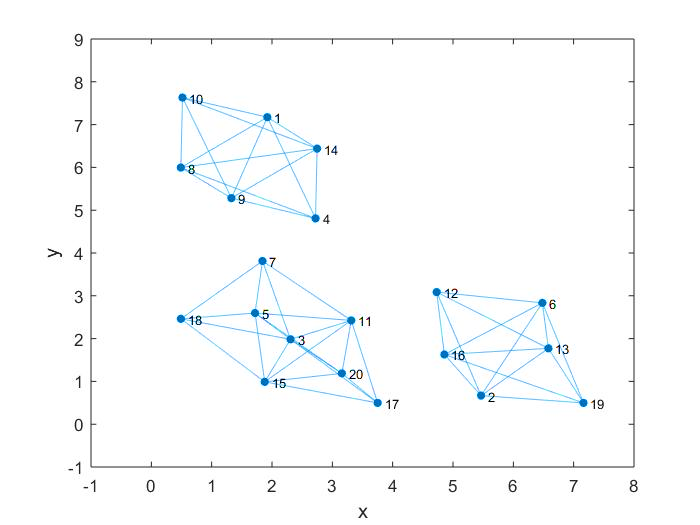
\includegraphics[width=0.5\linewidth]{graph.png}
    \caption{An example of the neighborhood graph representation among cluster centroids}
    \label{fig:graph}
\end{figure}

A community is a section (subgraph), which has higher internal density and lower external density with other sections. 
intra- and inter-cluster density
The cluster centroids in each community have more influence on each other than other centroids in other sections. It is necessary to use the influence of the centroids based on their distance from each other in updating the parameters. 

Therefore, in the neighborhood graph, in updating the cluster’s mean, its centroid is adjusted according to Eq. (\ref{eq:cluster centroid}) and proportional to its distance from each neighbor, it moves a certain amount closer to the centroid of that neighbor.
\begin{equation}\label{eq:cluster centroid}
    \hat{\mu}_i = \frac{\sum_{j=1}^{N_i}w_j \mu_j}{\sum_{j=1}^{N_i}w_j}, \quad w_j = \exp(-\beta d_{ij})
\end{equation}

Where $\hat{\mu}_i$ represents the centroid of cluster $i$ after the neighborhood operation, $N_i$ denotes the number of neighbors of the centroid of cluster $i$ and $\mu_j$ represents the centroid of cluster $j$. Additionally, $w_j$ denotes the neighborhood weight for the cluster centroid $j$. Where in that relation, $d_ij$ denotes the distance of the $j-th$ cluster centroid from the $i-th$ cluster centroid based on the feature vectors. Furthermore, $\beta$ is a constant, empirically chosen for each dataset, used to prevent a high impact from one cluster centroid on another.

This approach limits the significant impact of outlier data points entering the system on cluster centroids. By moving closer to neighboring centroids, its abrupt change is controlled, ultimately leading to a more robust clustering

\subsection{Rating prediction based on cluster membership and recommendation}
Following the clustering of users based on their ratings and feature vectors, in the test phase,the next step is to predict each user's rating for a given item. If the target user is already part of the system, their cluster membership have been previously determined. For new users, these degrees are computed using the method outlined in the previous section. Once the user’s cluster are determined, the predicted rating for a specific item is obtained as in Eq. \ref{eq:avgrating} by averaging the ratings given to that item by the user’s neighbors within the relevant clusters.

\begin{equation}\label{eq:avgrating}
    \frac{1}{C \times M} \sum_{k=1}^{C} \sum_{j=1}^{M} r_{kj}
\end{equation}

Finally, after predicting the scores for each user-item pair, items with the highest predicted scores are selected for recommendation. In most recommender systems, it is common to recommend the top 5 or 10 items. In the proposed recommender system, the top 5 items with the highest predicted ratings are recommended to each user.

\begin{figure}
    \centering
    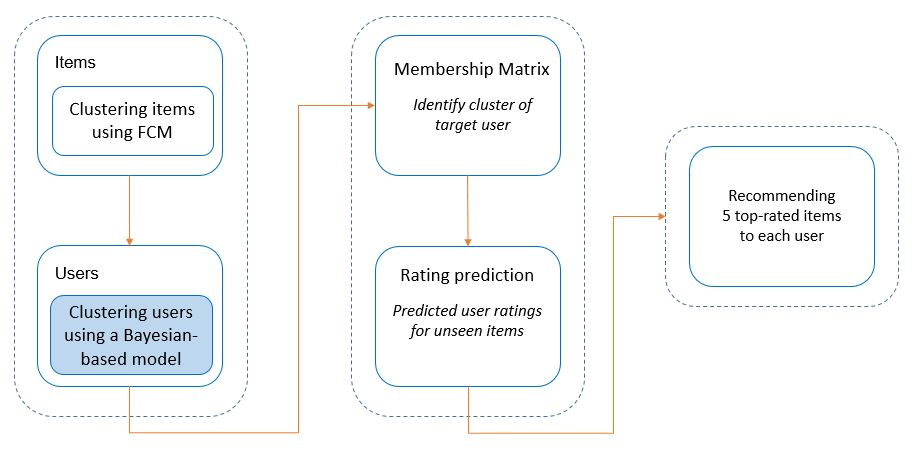
\includegraphics[width=0.9\linewidth]{flow.JPG}
    \caption{Flowchart of the recommender system, this study propose a bayesian-based user clustering method.}
    \label{fig:recommender_flow}
\end{figure}


\subsubsection{Convergence of the proposed method}
According to the theorem of \cite{hathaway1986local}, for a constant $m>1$, the corresponding FCM algorithm is locally converge to every minimum point $(U^*, \mu^*)$ of $J_m$ provided that the Hessian matrix of $Jm$ is positive definite in all feasible directions. 
% This states that, the iterations of the FCM algorithm cannot fluctuate within the same neighborhood. 
Hence, according to objective function defined in \ref{eq:obj function}, Hessian matrix defined as :

\begin{equation}
H_J = \begin{bmatrix}
\frac{\partial^2 J}{\partial u_{11}^2} & \frac{\partial^2 J}{\partial u_{11} \partial u_{12}} & \cdots & \frac{\partial^2 J}{\partial u_{11} \partial u_{NC}} & \frac{\partial^2 J}{\partial u_{11} \partial \theta_1} & \cdots & \frac{\partial^2 J}{\partial u_{11} \partial \theta_C} \\
\frac{\partial^2 J}{\partial u_{12} \partial u_{11}} & \frac{\partial^2 J}{\partial u_{12}^2} & \cdots & \frac{\partial^2 J}{\partial u_{12} \partial u_{NC}} & \frac{\partial^2 J}{\partial u_{12} \partial \theta_1} & \cdots & \frac{\partial^2 J}{\partial u_{12} \partial \theta_C} \\
\vdots & \vdots & \ddots & \vdots & \vdots & \ddots & \vdots \\
\frac{\partial^2 J}{\partial u_{NC} \partial u_{11}} & \frac{\partial^2 J}{\partial u_{NC} \partial u_{12}} & \cdots & \frac{\partial^2 J}{\partial u_{NC}^2} & \frac{\partial^2 J}{\partial u_{NC} \partial \theta_1} & \cdots & \frac{\partial^2 J}{\partial u_{NC} \partial \theta_C} \\
\frac{\partial^2 J}{\partial \theta_1 \partial u_{11}} & \frac{\partial^2 J}{\partial \theta_1 \partial u_{12}} & \cdots & \frac{\partial^2 J}{\partial \theta_1 \partial u_{NC}} & \frac{\partial^2 J}{\partial \theta_1^2} & \cdots & \frac{\partial^2 J}{\partial \theta_1 \partial \theta_C} \\
\vdots & \vdots & \ddots & \vdots & \vdots & \ddots & \vdots \\
\frac{\partial^2 J}{\partial \theta_C \partial u_{11}} & \frac{\partial^2 J}{\partial \theta_C \partial u_{12}} & \cdots & \frac{\partial^2 J}{\partial \theta_C \partial u_{NC}} & \frac{\partial^2 J}{\partial \theta_C \partial \theta_1} & \cdots & \frac{\partial^2 J}{\partial \theta_C^2}
\end {bmatrix}
\end{equation}

Then, to demonstrate that the Hessian matrix $H_J$ is positive definite, we need to show that for every non-zero vector $x$, the value of $x^TH_Jx$ is positive \cite{bhatia2009positive}. 
The $x^TH_Jx$ matrix includes four type of elements. 

The expressions \ref{eq:mat00} and \ref{eq:mat01} are equal to zero:

\begin{equation}\label{eq:mat00}
x_k \frac{\partial^2 J}{\partial u_{ij} \partial u_{lh}} x_g = 0 \quad \forall i \ne l, \, j \ne h 
\end{equation}

\begin{equation}\label{eq:mat01}
x_k \frac{\partial^2 J}{\partial u_{ij} \partial \theta_l} x_g = x_k \frac{\partial^2 J}{\partial \theta_l \partial u_{ij}} x_g = 0 \quad \forall j \ne l
\end{equation}

According to equations \ref{eq:xk0} and \ref{eq:xk0}, the values of expressions \ref{eq:mat00} and \ref{eq:mat00} are equal to zero, respectively. 

\begin{equation}\label{eq:xk0}
x_k \frac{\partial^2 J}{\partial u_{ij} \partial u_{lh}} x_g = x_k \left[ \frac{\partial (m u_{ij}^{m-1} f(\theta_j \mid z_i))}{\partial u_{lh}} \right] x_g = 0
\end{equation}

\begin{equation}\label{eq:xk00}
x_k \frac{\partial^2 J}{\partial u_{ij} \partial \theta_l} x_g = x_k \left[ \frac{\partial (m u_{ij}^{m-1} f(\theta_j \mid z_i))}{\partial \theta_l} \right] x_g = 0 
\end{equation}

Also, the values of expressions like \ref{eq:pos1} and \ref{eq:pos2} are positive:
\begin{equation}\label{eq:pos1}
x_k \frac{\partial^2 J}{\partial u_{ij}^2} x_k = x_k^2 m (m-1) u_{ij}^{m-2} f(\theta_j | z_i) \geq 0    
\end{equation}

\begin{equation}\label{eq:pos2}
\begin{aligned}
x_{NC+j} \frac{\partial^2 J}{\partial \theta_j^2} x_{NC+j} &= \sum_{i=1}^{N} \frac{u_{ij}^m}{(2\pi)^{1/2} |\Sigma_j|^{1/2} |\Sigma_{\theta_j}|^{1/2}} \\
&\quad \times \left[ \Sigma_j^{-1}(z_i - \mu_j) + \Sigma_{\theta_j}^{-1}(\mu_i - \mu_{\theta_j}) \right]^2 \\
&\quad \times \exp\left( -\frac{1}{2} \left( (z_i - \mu_j)^T \Sigma_j^{-1} (z_i - \mu_j) + (\mu_j - \mu_{\theta_j})^T \Sigma_{\theta_j}^{-1} (\mu_i - \mu_{\theta_j}) \right) \right) \geq 0
\end{aligned}
\end{equation}

In Equation \ref{eq:pos1}, since \( m > 1 \), it follows that \( m - 1 > 0 \). Also, \( u_{ij} \geq 0 \) because \( u_{ij} \) represents a membership degree, which can only be 0 or 1. Furthermore, \( f(\theta_j \mid x_i) \geq 0 \) as \( f \) is a posterior distribution function and therefore represents a probability.

In Eq. \ref{eq:pos2}, in the first term, since the covariance matrix is symmetric and positive semi-definite, then \( |\Sigma_j|^{1/2} \) and \( |\Sigma_{\theta_j}|^{1/2} \) are positive, because the determinant of a matrix is the product of its eigenvalues, and in a positive semi-definite matrix, the eigenvalues are non-negative. The second and third terms are positive due to the squared terms and the exponential function.

Additionally, the sum of similar terms such as in Eq. \ref{eq:xk00} also results in zero:

\begin{equation}
\begin{aligned}
& x_{NC+k} \frac{\partial^2 J}{\partial u_{ij} \partial \theta_j} x_g + x_g \frac{\partial^2 J}{\partial \theta_j \partial u_{ij}} x_{NC+k} \\
= & \, x_{NC+k} x_g \frac{m u_{ij}^{m-1}}{2\pi |\Sigma_{\theta_j}|^{1/2}} f_{ij} \Bigg[ |\Sigma_j|^{-5/2} \Sigma_j^{-T} \Sigma_j^{-1} (z_i - \mu_j) + |\Sigma_j|^{-5/2} \Sigma_j^{-T} \Sigma_{\theta_j}^{-1} (\mu_i - \mu_{\theta_j}) \\
& \quad - \frac{1}{|\Sigma_j|^{1/2}} \Sigma_j^{-1} (z_i - \mu_j)^T \Sigma_j^{-1} + \frac{1}{|\Sigma_j|^{1/2}} \left( \Sigma_j^{-1}(z_i - \mu_j) + \Sigma_{\theta_j}^{-1}(\mu_i - \mu_{\theta_j}) \right)^2 \\
& \quad - |\Sigma_j|^{-5/2} \Sigma_j^{-T} \Sigma_j^{-1}(z_i - \mu_j) - \frac{1}{|\Sigma_j|^{1/2}} \left( \Sigma_j^{-1}(z_i - \mu_j) + \Sigma_{\theta_j}^{-1}(\mu_i - \mu_{\theta_j}) \right)^2 \\
& \quad - |\Sigma_j|^{-5/2} \Sigma_j^{-T} \Sigma_{\theta_j}^{-1}(\mu_i - \mu_{\theta_j}) + \frac{1}{|\Sigma_j|^{1/2}} \Sigma_j^{-1}(z_i - \mu_j)^T \Sigma_j^{-1} \Bigg] = 0
\end{aligned}
\end{equation}

Finally, by substituting the expressions, the $x^TH_Jx$ matrix is obtained as:
\begin{equation} \label{eq:Hessian2}
\begin{aligned}
x H_J^T x = & \hspace{1.2em} \left[ x_1 \frac{\partial^2 J}{\partial u_{11}^2} x_1 + 0 + \hspace{1.45em} \cdots \quad + 0 + x_{NC+1} \frac{\partial^2 J}{\partial \theta_1 \partial u_{11}} x_1 + 0 + \hspace{1.45em} \cdots \quad + 0 \right] \\
& + \left[ 0 + x_2 \frac{\partial^2 J}{\partial u_{12}^2} x_2 + 0 + \quad \cdots \hspace{0.6em} + 0 + x_{NC+2} \frac{\partial^2 J}{\partial \theta_2 \partial u_{12}} x_2 + 0 +\quad \cdots \hspace{0.6em} + 0 \right] \\ 
& + \cdots \\ \hfill
& + \left[ 0 + \cdots + 0 + x_{NC} \frac{\partial^2 J}{\partial u_{NC}^2} x_{NC} + 0 +\hspace{1.34em} \cdots + 0 + x_{NC+C} \frac{\partial^2 J}{\partial \theta_C \partial u_{NC}} x_{NC} \right] \\ \hfill
& + \left[ x_1 \frac{\partial^2 J}{\partial u_{11} \partial \theta_1} x_{NC+1} + 0 + \quad \cdots + 0 + x_{NC+1} \frac{\partial^2 J}{\partial \theta_1^2} x_{NC+1} + 0 + \quad \cdots + 0 \right] \\ \hfill
& + \cdots \\
& + \left[ 0 + \cdots + 0 + x_{NC} \frac{\partial^2 J}{\partial u_{NC} \partial \theta_C} x_{NC+C} + 0 + \cdots + 0 + x_{NC+C} \frac{\partial^2 J}{\partial \theta_C^2} x_{NC+C} \right] \\
& \geq 0
\end{aligned}
\end{equation}

The positivity of Eq. \ref{eq:Hessian2} confirms that the Hessian matrix of function $H_J$ is positive definite in all directions.
The theorem of \cite{hathaway1986local} implies that if the clustering algorithm starts with points sufficiently close to the minimum of the objective function, it will converge after iterations. Since the proposed method utilizes prior knowledge, an initial clustering is performed based on the available data. This step ensures that the algorithm begins near the minimum point of the objective function, thereby it guarantees convergence.

\subsubsection{Convergence rate of proposed method}

To determine the convergence rate of the proposed clustering algorithm, the variations of cluster centroids across consecutive iterations were analyzed. First, we show that equation (29), which defines the cluster centroids, is a recursive relation based on the cluster centroids in the previous iteration:

\begin{equation}
\mu_{n+1} = \left( \frac{\Sigma_j^{-1}}{\Sigma_j^{-1} + \Sigma_{\theta_j}^{-1}} \right) \left( \frac{\sum_{i=1}^{n} u_{ij}^m f_{ij} x_i}{\sum_{i=1}^{n+1} u_{ij}^m f_{ij}} + \frac{u_{(n+1)j}^m f_{(n+1)j} x_{n+1}}{\sum_{i=1}^{n+1} u_{ij}^m f_{ij}} \right) + \left( \frac{\Sigma_{\theta_j}^{-1}}{\Sigma_j^{-1} + \Sigma_{\theta_j}^{-1}} \right) \frac{\sum_{i=1}^{n} u_{ij}^m f_{ij} \mu_{\theta_j}}{\sum_{i=1}^{n+1} u_{ij}^m f_{ij}}
\end{equation}
this leads to the following simplified form:
\begin{equation}
\mu_{n+1} = \mu_n \cdot S + x_{n+1} \cdot (1 - S) + M
\end{equation}
where
\begin{equation}
S = \frac{\sum_{i=1}^{n} u_{ij}^m f_{ij}}{\sum_{i=1}^{n+1} u_{ij}^m f_{ij}}, \quad 
1 - S = \frac{u_{(n+1)j}^m f_{(n+1)j}}{\sum_{i=1}^{n+1} u_{ij}^m f_{ij}}, \quad 
M = \left( \frac{\Sigma_{\theta_j}^{-1}}{\Sigma_j^{-1} + \Sigma_{\theta_j}^{-1}} \right) \frac{\sum_{i=1}^{n} u_{ij}^m f_{ij} \mu_{\theta_j}}{\sum_{i=1}^{n+1} u_{ij}^m f_{ij}}
\end{equation}

The differential of \( \mu(k) \) is considered, to investigate the change in cluster centroids during each iteration. Based on the recursive equation for the cluster centroid, the variation resembles the capacitor discharge equation. According to Kirchhoff's law, the voltage drop across a resistor-capacitor circuit is modeled by a first-order differential equation:

\begin{equation}
\frac{Q}{C} + R \frac{dQ}{dt} = 0 \Rightarrow \frac{dQ}{dt} = -\frac{Q}{\tau}, \quad \text{where } \tau = RC
\end{equation}
integrating both sides yields:

\begin{equation}
\int_{Q=Q_0}^{Q=Q(t)} \frac{dQ}{Q} = - \int_{t=0}^{t} \frac{dt}{\tau}
\end{equation}

\begin{equation}
\ln\left[\frac{Q(t)}{Q_0}\right] = -\frac{t}{\tau}
\end{equation}

Similar to the capacitor discharge equation, the differential of \( \mu(k) \) in the continuous case becomes:

\begin{equation}
\frac{d\mu}{dt} = -\frac{\mu}{\tau}
\end{equation}
integrating leads to:

\begin{equation}
\mu(k) = \mu(0) e^{-t / \tau}
\end{equation}
in the discrete case:

\begin{equation}
\frac{\mu(k) - \mu(0)}{k} = -\frac{\mu(k)}{\tau} \Rightarrow 
\tau_\mu = \frac{-k \mu(k)}{\mu(k) - \mu(0)}
\end{equation}
then, \( \mu(k) \) is obtained recursively as:

\begin{equation}\label{eq: mu(k)}
    \mu(k) = \mu(0) + \sum_{i=1}^{k} S^{k - i}(1 - S)x(i) + M, \quad M \triangleq kM
\end{equation}


substituting $\mu(k)$ into Eq. \ref{eq: mu(k)}, have:

\begin{equation}
\tau_\mu = \frac{-k \mu(0)}{\sum_{i=1}^{k} S^{k - i}(1 - S)x(i) + M} + k
\end{equation}

Finally, substituting this into, the exponential model for the variation of cluster centroids in the proposed method is obtained as:
\begin{equation}
\mu(k) = \mu(0) e^{{-t}/{\frac{-k \mu(0)}{\sum_{i=1}^{k} S^{k - i}(1 - S)x(i) + M} + k}}
\end{equation}


\begin{figure}
\centering
% Subfigure 1
\begin{subfigure}[b]{0.45\textwidth}
    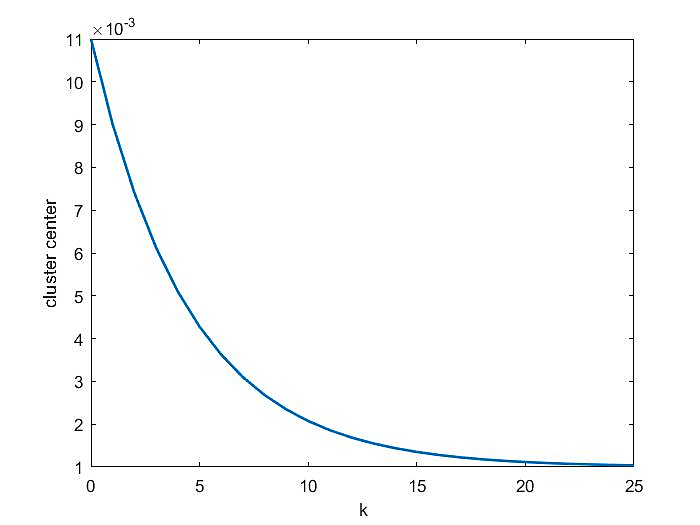
\includegraphics[width=\textwidth]{Cnrate_FCM.png}
    \caption{FCM}
    % \label{fig:sub1}
\end{subfigure}
% \hfill
% Subfigure 2
\begin{subfigure}[b]{0.45\textwidth}
    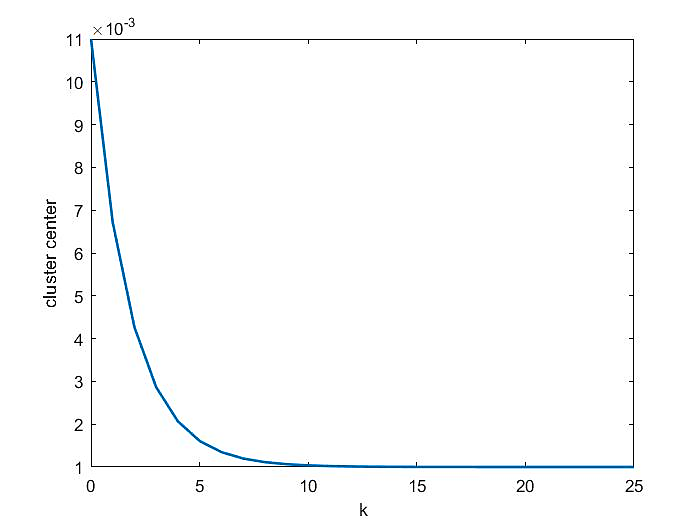
\includegraphics[width=\textwidth]{Cnrate_pmethod.png}
    \caption{Proposed method}
    % \label{fig:sub2}
\end{subfigure}
\caption{Comparison of convergence rates of the proposed clustering method and FCM method}
\label{fig:cn-rate}
\end{figure}


In Figure \ref{fig:cn-rate}, the exponential models of the proposed method and the FCM method are compared. The figure indicates that the cluster centroids in the proposed method change more rapidly, resulting in a faster convergence compared to FCM.

% ************************************************************************

\section{Experiments}
In this section, we investigate the accuracy and performance of the proposed method on various datasets. A comparative analysis with other methods as well as a discussion in parameter setting  is presented.

\subsection{Data sets}
The proposed recommender system was evaluated on the widely used MovieLens-100k, and MovieLens-1M and Yelp datasets, which are standard benchmarks in recommender system methods.
The MovieLens dataset includes user ratings and movie features collected from the MovieLens website, with movies categorized by genre. Preprocessing converted genres into binary indicators, where 1 denotes genre membership and 0 otherwise. The study utilizes MovieLens 100K, which includes 100,000 ratings from 1,000 users across 1,700 movies, and MovieLens 1M, containing 1 million ratings from 6,000 users for 4,000 movies, with additional user attributes such as age, gender, and occupation. These attributes are used for clustering in recommendation models.

The Yelp dataset features information on businesses across 11 cities in 4 countries, focusing on the restaurant category. It includes 4 million reviews from 1 million users for 58,000 restaurants, with detailed restaurant features (e.g., parking, child-friendliness, ambiance) and user attributes (e.g., age, gender, and average rating). Restaurant features were converted into numerical values (0 for absence, 1 for presence, and -1 for unspecified).

\subsection{Evaluation criteria}
Recommender systems are typically evaluated using two categories of criteria, prediction accuracy and decision support. Prediction accuracy metrics, such as Mean Absolute Error (MAE) and Root Mean Squared Error (RMSE), measure the numerical accuracy of predicted ratings. 

\begin{equation}
    \text{MAE} = \frac{1}{|S|} \sum_{i=1}^{|S|} |pred_i - r_i|
\end{equation}


\begin{equation}
    \text{RMSE} = \sqrt{\frac{1}{|S|} \sum_{i=1}^{|S|} (pred_i - r_i)^2}
\end{equation}

where, $pred_i$ and $r_i$ are the predicted and real scores for item $i$ respectively, and $|S|$ is number of test data.

In contrast, decision support metrics, including precision, recall, and F1 score, evaluate the system's effectiveness in providing relevant recommendations. Predicted scores for the items determined whether an item should be considered relevant and recommended to the target user or not. With a score range of 1 to 5, items rating $\leq 3$ are classified as irrelevant, while those rating $\geq 4$ are considered relevant. Therefore, precision, defined as the ratio of relevant suggested items to the total suggested items, ensures that recommendations are relevant and minimize unnecessary suggestions. Recall is the ratio of suggested relevant items to the total number of relevant items. F1 is a combination of precision and recall. These are defined as follows
\[
\text{Precision} = \frac{\#tp}{\#tp + \#fp}
\]

\[
\text{Recall} = \frac{\#tp}{\#tp + \#fn}
\]

\[
F1 = \frac{2 \times P \times R}{P + R}
\]
where, tp denotes the items suggested to the user by the recommendation system based on the predicted score, that are also relevant according to the actual score. Similarly, fp , fn and tn represent the suggested irrelevant items, not suggested relevant items and not suggested irrelevant items, respectively.


\subsection{Evaluation of the Proposed Recommender System}
To assess the accuracy of the proposed recommender system and compare the effectiveness of the proposed approach, its performance was benchmarked against existing clustering-based recommendation methods, including \cite{liji2018improved, kant2017leaderrank, mohammadpour2019efficient, wasid2018clustering}. Table \ref{tab:comparison_results} presents the comparison results for different methods using the evaluation criteria on the MovieLens-100K, MovieLens-1M, and Yelp datasets.

\begin{table}[htbp]
\centering
\caption{Comparison of the Proposed Method with others}
\label{tab:comparison_results}
\renewcommand{\arraystretch}{1.3}
\setlength{\tabcolsep}{3pt}
\begin{tabular}{clccccc}
\hline
\textbf{Data Sets} & \textbf{Method} & \textbf{MAE} & \textbf{RMSE} & \textbf{Precision} & \textbf{Recall} & \textbf{F1} \\
\hline
\multirow{5}{*}{ML\_100K} & Chen\cite{liji2018improved} & 0.74 & 0.95 & 0.88 & 0.50 & 0.642 \\
& Kant\cite{kant2017leaderrank} & 0.75 & 0.95 & 0.56 & 0.87 & 0.681 \\
& Enayatifar \cite{mohammadpour2019efficient} & 0.78 & 0.96 & - & - & - \\
& Wasid \cite{wasid2018clustering} & 0.91 & 1.12 & 0.54 & 0.75 & 0.627 \\
& \textbf{Proposed Method} & \textbf{0.71} & \textbf{0.91} & 0.56 & 0.89 & \textbf{0.687} \\
\hline
\multirow{5}{*}{ML\_1M} & Chen & 0.72 & 0.94 & 85.3 & 0.49 & 0.622 \\
& Kant & 0.72 & 0.925 & 0.53 & 0.86 & 0.653 \\
& Enayatifar & 0.85 & 1.35 & - & - & - \\
& Wasid & 0.95 & 1.24 & 0.56 & 0.71 & 0.626 \\
& \textbf{Proposed Method} & \textbf{0.705} & \textbf{0.925} & 0.62 & 0.85 & \textbf{0.71} \\
\hline
\multirow{3}{*}{Yelp} & Kant & 0.965 & 1.25 & 0.57 & 0.78 & 0.65 \\
&  \textbf{Proposed Method} & \textbf{0.943} & \textbf{1.21} & 0.61 & 0.81 & \textbf{0.69} \\
\hline
\end{tabular}
\end{table}

In all the mentioned methods, a clustering model has been used to find users or similar items and finally predict the score for the users. Also, in all these studies, the number of data has been assumed to be constant. According to the comparison, it is observed that although the proposed method considers the data as online and streaming, it has better performance than other methods.

Furthermore, to evaluate the feasibility of the proposed method for real-time applications, we analyzed the computation time required for rating predictions. Table \ref{tab:computation_time} presents the comparison between the proposed method and the approach \cite{kant2017leaderrank} in terms of maximum computational time required per prediction in three datasets. It is evident that the proposed method performs efficiently compared to existing approaches. Its speed makes it suitable for deployment in real-world systems with streaming data.

\begin{table}[h]
\centering
\caption{Computational Time Comparison (in milliseconds)}
\label{tab:computation_time}
\renewcommand{\arraystretch}{1.3}
% \setlength{\tabcolsep}{2pt}
\begin{tabular}{lccc}
    \hline
    \textbf{Method} & \textbf{Yelp} & \textbf{MovieLens-100K} & \textbf{MovieLens-1M} \\
    \hline
    Kant et al. [43] & 48 ms & 18 ms & 25 ms \\
    \textbf{Proposed Method} & \textbf{50 ms} & \textbf{22 ms} & \textbf{28 ms} \\
    \hline
\end{tabular}
\end{table}

\subsection{comparision with standard FCM}

For comparing the final performance and convergence speed of the proposed clustering method versus the standard FCM, the FCM objective function's value is computed separately for both methods per iteration. This allows for a proper comparison, even though each method updates parameters differently and has its own unique objective function. The convergence speed comparison for every dataset can be seen in Figure \ref{fig:combined}.

\begin{figure}[H]
\centering
% Subfigure 1
\begin{subfigure}[b]{0.3\textwidth}
    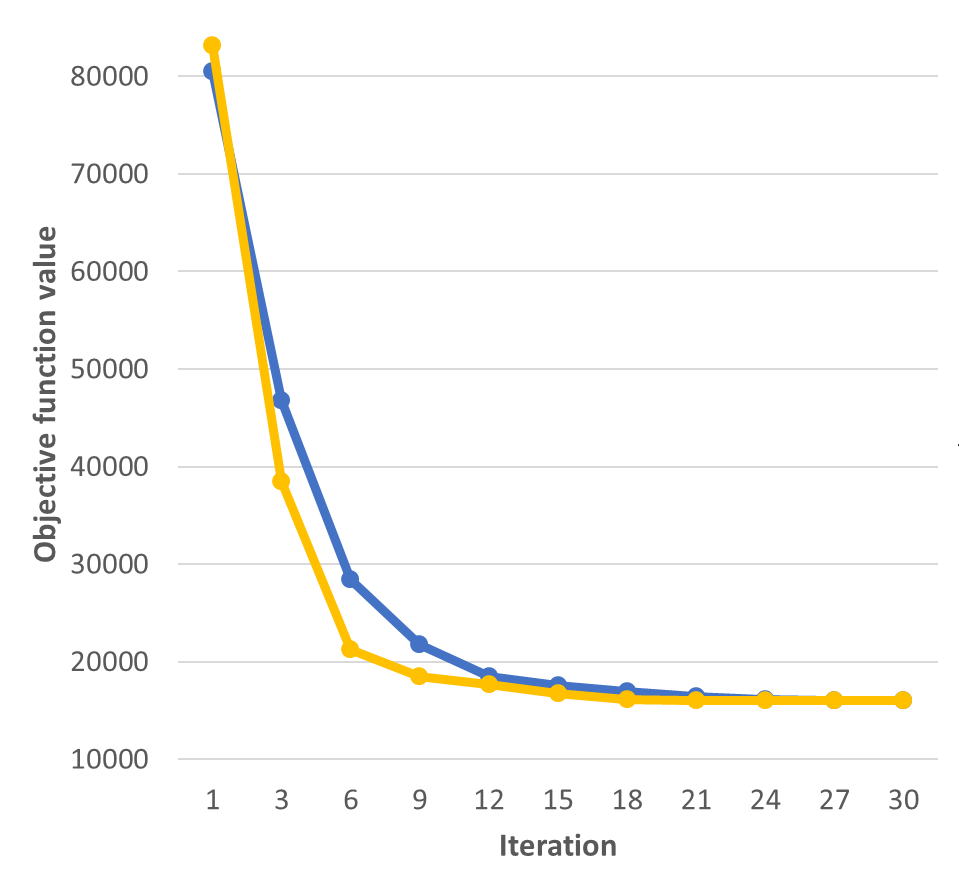
\includegraphics[width=\textwidth]{fcm1final.png}
    \caption{M\_100K}
    % \label{fig:sub1}
\end{subfigure}
\hfill
% Subfigure 2
\begin{subfigure}[b]{0.3\textwidth}
    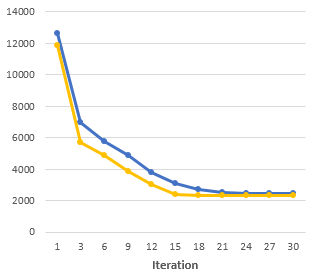
\includegraphics[width=\textwidth]{fcm2final.PNG}
    \caption{ML\_1M}
    % \label{fig:sub2}
\end{subfigure}
\hfill
% Subfigure 3
\begin{subfigure}[b]{0.3\textwidth}
    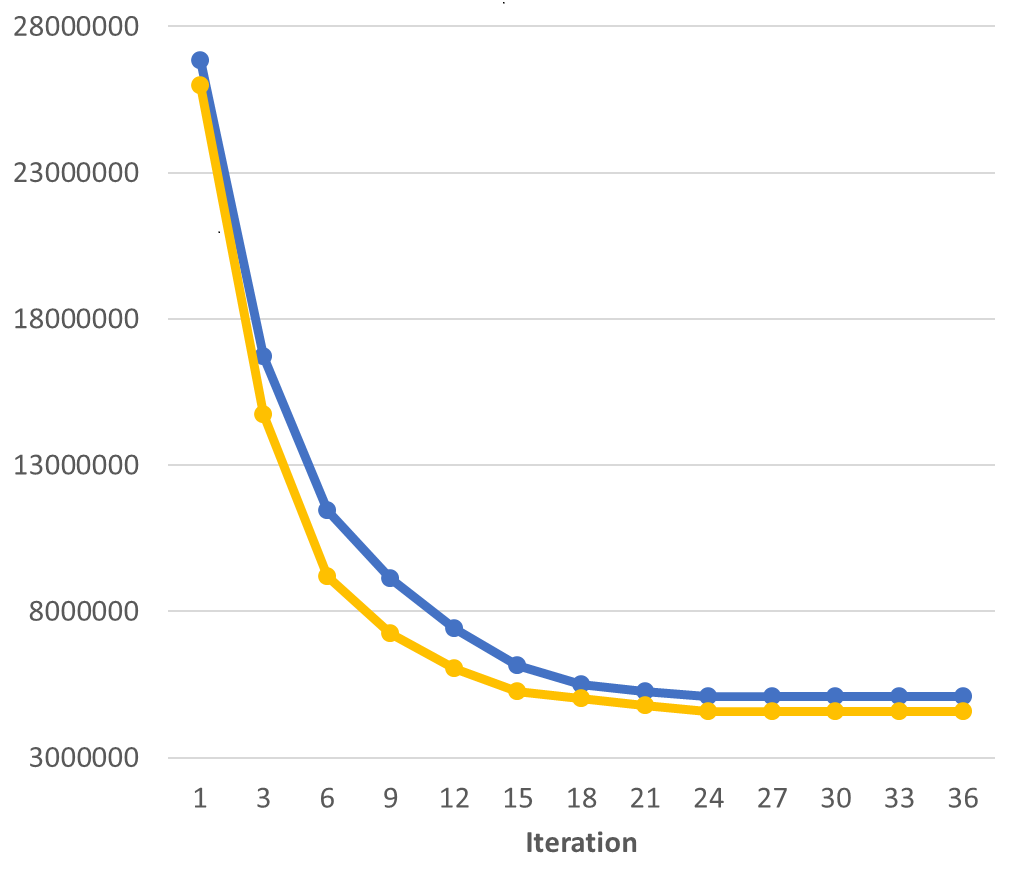
\includegraphics[width=\textwidth]{fcm3final.png}
    \caption{Yelp}
    % \label{fig:sub3}
\end{subfigure}

\caption{Comparison of the convergence rate and speed of the proposed method and the FCM method on the different datasets. Blue and yellow line denotes the FCM and proposed method respectively}
\label{fig:combined}
\end{figure}


Table \ref{tab:cmpFCM} compares both methods based on the minimum FCM objective function value attained and the minimum iterations required. The comparison demonstrates that the proposed method outperforms FCM by converging faster and lowering the objective function value more substantially.

\begin{table}[htbp]
\centering
\caption{Comparison of the proposed method with FCM}
\label{tab:cmpFCM}
\renewcommand{\arraystretch}{1.3}
\setlength{\tabcolsep}{8pt}
\begin{tabular}{lcccc}
\hline
% \rowcolor[gray]{0.9}
\textbf{Data set} & \multicolumn{2}{c}{\textbf{FCM}} & \multicolumn{2}{c}{\textbf{Proposed method}} \\
\cline{2-5}
& \textbf{value} & \textbf{iterations} & \textbf{value} & \textbf{iterations} \\
\hline
ML-100K & 2709 & 18 & 2402 & 15 \\
ML-1M   & 16099 & 22 & 16093 & 19 \\
% \rowcolor[gray]{0.9}
Yelp    & 5078242 & 26 & 4587557 & 23 \\
\hline
\end{tabular}
\end{table}



\subsection{Parameter Discussion}
To assess the effect of different parameter settings on performance, we conducted experiments to analyze the impact of number of cluster and the percentage of data used in initial clustering. 
Initially, 80\% of the data is randomly selected as training data, while the remaining 20\% is used for testing.
Then, a portion of the training data is allocated for initial clustering and parameter setting. Consequently, both the number of user clusters and the proportion of data used for this initial phase influence the quality of the clustering results.
Table \ref{tab:parameter_discussion} presents the prediction accuracy of the proposed recommender system across different numbers of user clusters and considering two data usage scenarios: 30\% and 40\% of the training data.

The results indicate that using 40\% of the data for initial clustering leads to more effective user clustering, which enhances the overall prediction accuracy.

\begin{table}[htbp]
\centering
\caption{Accuracy of the proposed method across different parameter settings}
\label{tab:parameter_discussion}
\renewcommand{\arraystretch}{1.3}
\setlength{\tabcolsep}{3pt}
\begin{tabular}{cccccccccc}
\hline
\multirow{2}{*}{\textbf{Datasets}} & \multirow{2}{*}{\begin{tabular}[c]{@{}c@{}} initial \\ data\end{tabular}} & \multicolumn{2}{c}{\textbf{60}} & \multicolumn{2}{c}{\textbf{80}} & \multicolumn{2}{c}{\textbf{100}} & \multicolumn{2}{c}{\textbf{110}} \\
\cline{3-10}
 &  & MAE & RMSE & MAE & RMSE & MAE & RMSE & MAE & RMSE \\
\hline
\multirow{2}{*}{ML\_100K} & 30\% & 0.73 & 0.925 & 0.72 & 0.92 & 0.76 & 0.955 & - & - \\
 & 40\% & 0.73 & 0.917 & \textbf{0.71} & \textbf{0.91} & 0.74 & 0.96 & - & - \\
\hline
\multirow{2}{*}{ML\_1M} & 30\% & 0.78 & 1.0 & 0.763 & 0.979 & 0.72 & 0.95 & 0.725 & 0.935 \\
 & 40\% & 0.77 & 0.98 & 0.752 & 0.976 & \textbf{0.705} & \textbf{0.925} & 0.718 & 0.93 \\
\hline
\multirow{2}{*}{Yelp} & 30\% & 0.993 & 1.45 & 0.975 & 1.43 & 0.965 & 1.31 & 0.955 & 1.32 \\
 & 40\% & 0.99 & 1.47 & 0.965 & 1.40 & 0.945 & 1.25 &\textbf{0.943} &\textbf{1.21} \\
\hline
\end{tabular}
\end{table}


In addition, based on these comparisons, the optimal number of clusters for users in each data set is determined. According to the results obtained, the optimal number of clusters for the MovieLens\_100k data set is 80 clusters, for the MovieLens\_1M data set is 100 clusters, and for the yelp data set is 110 clusters.

Also, according to the experiments conducted, the optimal number of clusters for items in the MovieLens dataset, due to the limited number of genres, was 20 clusters and in the Yelp dataset, 80 clusters.

These findings confirm that the proposed Bayesian clustering model outperforms traditional clustering approaches while maintaining low computational overhead, making it well-suited for real-time recommender systems.

\section{Conclusion}
In this study, a method based on the Bayesian clustering model is used. Initially, to reduce the feature for user clustering, the items are clustered using FCM. Then, As considering the users are not constant and added to the system dynamically, a Bayesian clustering method is used for user clustering. In this approach, learning is conducted in a distributed manner, where cluster centroids interact and influence each another based on their relative distances. This minimizes the impact of outliers on the cluster centroids. Finally, after clustering, the scores of neighboring users are used to predict a user's score on an item that they have not seen yet, and the items with the highest scores are suggested to each user. The evaluation results on streaming data events demonstrate that the proposed method outperforms existing approaches in enhancing recommender system performance, achieving more precise user score predictions. In proposed method, items are considered constant, which is a limitation in real-world application. Future research could address this by considering dynamic item. Furthermore, integrating a score prediction methods that utilize both user-user and item-item similarities could enhance recommendation accuracy.

% \bibliographystyle{plain} % Specify the bibliography style
% \bibliography{RecommendationBib.bib}
\printbibliography

\end{document}

% F. Maxwell Harper and Joseph A. Konstan. The movielens datasets: Historyand context. ACM Trans. Interact. Intell.
Syst., 5(4):19:1–19:19, 2016.